\documentclass[aspectratio=169,11pt]{beamer}

% ============================================================
% PACKAGES
% ============================================================
\usepackage{graphicx}
\usepackage{tikz}
\usetikzlibrary{positioning,arrows.meta}
\usepackage{xcolor}
\usepackage{booktabs}
\usepackage{tabularx}
\usepackage{array}
\usepackage{ragged2e}
\usepackage{hyperref}

% ============================================================
% COLORS - SAME AS PHASE-I
% ============================================================
\definecolor{GEUBlue}{RGB}{20,55,105}
\definecolor{GEULightBlue}{RGB}{238,244,251}
\definecolor{GEUGrey}{RGB}{90,90,90}
\definecolor{GEULightGrey}{RGB}{245,246,248}

% ============================================================
% BEAMER SETTINGS
% ============================================================
\usetheme{default}
\setbeamertemplate{navigation symbols}{}
\setbeamertemplate{blocks}[rounded][shadow=false]

\setbeamercolor{normal text}{fg=black,bg=white}
\setbeamercolor{frametitle}{fg=GEUBlue}
\setbeamercolor{structure}{fg=GEUBlue}
\setbeamercolor{block title}{fg=GEUBlue,bg=GEULightBlue}
\setbeamercolor{block body}{fg=black,bg=GEULightBlue}

\setbeamerfont{frametitle}{size=\Large,series=\bfseries}

% ============================================================
% LOGO
% ============================================================
% Upload the Graphic Era logo with this filename to Overleaf.
\newcommand{\GEULogo}{graphicera_logo.png}

% ============================================================
% HEADER
% ============================================================
\setbeamertemplate{headline}{%
  \begin{tikzpicture}[remember picture,overlay]
    \node[
        anchor=north east,
        xshift=-0.30cm,
        yshift=-0.12cm
    ] at (current page.north east)
    {\includegraphics[height=0.62cm]{\GEULogo}};
  \end{tikzpicture}
  \vspace{0.72cm}
}

% ============================================================
% FRAME TITLE
% ============================================================
\setbeamertemplate{frametitle}{%
  \vspace{0.03cm}
  \insertframetitle\par
  \vspace{0.04cm}
  \textcolor{GEUBlue}{\rule{\textwidth}{0.9pt}}
  \vspace{0.03cm}
}

% ============================================================
% FOOTER
% ============================================================
\setbeamertemplate{footline}{%
  \leavevmode
  \hbox{%
  \begin{beamercolorbox}[
      wd=.82\paperwidth,
      ht=0.32cm,
      dp=0.10cm,
      leftskip=.3cm
  ]{author in head/foot}
    \tiny Department of Computer Science \& Engineering |
    Graphic Era (Deemed to be University)
  \end{beamercolorbox}%
  \begin{beamercolorbox}[
      wd=.18\paperwidth,
      ht=0.32cm,
      dp=0.10cm,
      rightskip=.3cm
  ]{date in head/foot}
    \hfill\tiny\insertframenumber/\inserttotalframenumber
  \end{beamercolorbox}}
}

% ============================================================
% CUSTOM COMMANDS
% ============================================================
\newcommand{\smallnote}[1]{%
\vspace{0.08cm}
{\scriptsize\color{GEUGrey}#1}
}

\newcommand{\placeholder}[1]{%
\textit{\color{GEUGrey}#1}
}

% ============================================================
% DOCUMENT INFORMATION
% ============================================================
\title{\textbf{Project-Based Learning}\\[2mm]\large Phase-II Evaluation}
\author{\textbf{Project Title}\\Team ID: XXXX}

\institute{
Department of Computer Science \& Engineering\\
Graphic Era (Deemed to be University), Dehradun
}

\date{Academic Session 2026--27}

% ============================================================
% DOCUMENT
% ============================================================
\begin{document}

% ============================================================
% SLIDE 1
% ============================================================
\begin{frame}[plain]

\begin{tikzpicture}[remember picture,overlay]

\draw[GEUBlue,line width=3pt]
(current page.north west) -- (current page.north east);

\node[
    anchor=north east,
    xshift=-0.45cm,
    yshift=-0.35cm
] at (current page.north east)
{\includegraphics[height=1.0cm]{\GEULogo}};

\node[
    align=center,
    text width=.84\paperwidth
] at ([yshift=.25cm]current page.center)
{
{\color{GEUBlue}
\fontsize{26}{30}\selectfont
\bfseries PROJECT-BASED LEARNING}
\\[3mm]

{\fontsize{18}{22}\selectfont
PHASE-II EVALUATION}
\\[7mm]

{\color{GEUGrey}
\Large\bfseries
\placeholder{VidOptix -VideoCompressionSystem}}
\\[3mm]

{\color{GEUBlue}
\normalsize Team ID: DSCPP-III-2026-T198}
};

\node[
    align=center,
    anchor=south,
    yshift=.42cm
] at (current page.south)
{
\bfseries
Department of Computer Science \& Engineering\\
Graphic Era (Deemed to be University), Dehradun\\[-1mm]
\scriptsize Academic Session 2026--27
};

\end{tikzpicture}

\end{frame}

% ============================================================
% SLIDE 2
% ========================================================\begin{frame}{Team \& Mentor Details}

\begin{columns}[T,totalwidth=\textwidth]

\column{.48\textwidth}

\begin{block}{Team Information}
\begin{tabular}{@{}ll@{}}
\textbf{Team ID:} & DSCPP-III-2026-T198\\
\textbf{Semester:} & 3rd \\
\textbf{Section:} & B,DS1,ML1,ML2\\
\textbf{Domain:} & \placeholder{Data Structure and C++}
\end{tabular}
\end{block}

\column{.48\textwidth}

\begin{block}{Team Members}
1.\quad \placeholder{Anshika Goswami – 2510380062}\\
2.\quad \placeholder{Yaduveer Yadav – 2510370438}\\
3.\quad \placeholder{Deepanshi Choudhary – 2510370456}\\
4.\quad \placeholder{Mohd Ubaid – 2510370084}
\end{block}

\end{columns}

\vspace{2mm}

\begin{block}{Mentor}
\placeholder{Mr. Kartikey Arora }
\hfill
\textbf{Interactions completed: 4}
\end{block}

\vfill

\smallnote{
 BitSquad is developing VidOptix in the Data Structures and C++ domain,
our responsibilities include algorithm development,
video processing, enhancement, interface design,
and testing.
}

\end{frame}

% ============================================================
% SLIDE 3
% ============================================================
\begin{frame}{Phase-I Recap \& Feedback Incorporated}
\scriptsize

\begin{block}{Phase-I Status}
\placeholder{
The project was proposed as a frame-based video compression system intended to reduce video file size while keeping acceptable visual quality.
}
\end{block}

\vspace{2mm}

\begin{columns}[T,totalwidth=\textwidth]

\column{.48\textwidth}

\textbf{\color{GEUBlue}Feedback Received}
\begin{itemize}\itemsep2pt
\item \placeholder{ Improve quality preservation alongside compression.}
\item \placeholder{Complete the compression pipeline.}
\item \placeholder{Make the interface easier to use.}
\end{itemize}

\column{.48\textwidth}

\textbf{\color{GEUBlue}Changes Incorporated}

\begin{itemize}\itemsep2pt
\item \placeholder{Enhancement methods added to project scope.}
\item \placeholder{DCT / quantization / coding integration planned.}
\item \placeholder{UI workflow for settings and output preview planned.}
\end{itemize}

\end{columns}

\smallnote{
Brief Discussion:  Phase-II work focuses on incorporating quality preservation, optional enhancement, and a more complete workflow.
}

\end{frame}

% ============================================================
% SLIDE 4
% ============================================================
\begin{frame}{Problem Statement \& Finalized Objectives}

\begin{block}{Problem Statement}
\placeholder{
Video files require substantial storage. VidOptix aims to reduce video size through frame-based compression while maintaining acceptable visual quality and exploring enhancement techniques.
}
\end{block}

\vspace{2mm}

\textbf{\color{GEUBlue}Finalized Objectives}

\begin{enumerate}\itemsep3pt
\item \placeholder{Read video frames and divide them into 8×8 blocks.}
\item \placeholder{Apply DCT and integrate quantization, zig-zag scan, RLE and Huffman coding.}
\item \placeholder{ Provide optional enhancement and denoising.}
\item \placeholder{Evaluate file-size reduction, processing time and visual quality.}
\end{enumerate}

\vfill

\smallnote{
Brief Discussion: The finalized scope balances compression efficiency, visual quality and usability.
}

\end{frame}

% ============================================================
% SLIDE 5
% ============================================================
\begin{frame}{Updated System Architecture / Workflow}

\begin{center}

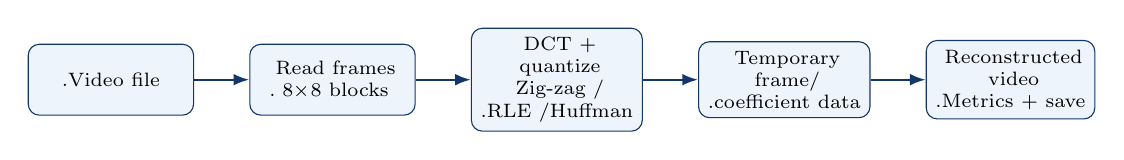
\begin{tikzpicture}[
node distance=7mm,
box/.style={
rectangle,
rounded corners,
draw=GEUBlue,
fill=GEULightBlue,
minimum width=2.10cm,
minimum height=9mm,
align=center,
font=\scriptsize.
},
arrow/.style={
-{Latex[length=2mm]},
thick,
draw=GEUBlue
}
]

\node[box] (a) {Video file};
\node[box,right=of a] (b) {Read frames\\
8×8 blocks};
\node[box,right=of b] (c) {DCT + \\quantize\\
Zig-zag /\\ RLE /Huffman};
\node[box,right=of c] (d) {Temporary \\frame/\\
coefficient data};
\node[box,right=of d] (e) {Reconstructed \\video\\
Metrics + save};

\draw[arrow] (a)--(b);
\draw[arrow] (b)--(c);
\draw[arrow] (c)--(d);
\draw[arrow] (d)--(e);

\end{tikzpicture}

\end{center}

\vspace{0.2mm}

\begin{columns}[T,totalwidth=\textwidth]

\column{.48\textwidth}

\textbf{\color{GEUBlue}Major Components}

\begin{itemize}\itemsep-2pt
\item \placeholder{Frame reader and extractor}
\item \placeholder{8×8 block DCT and compression stages}
\item \placeholder{Optional enhancement / denoising}
\end{itemize}

\column{.48\textwidth}

\textbf{\color{GEUBlue}Changes Since Phase-I}

\begin{itemize}\itemsep-2pt
\item \placeholder{Quality preservation is an explicit focus.}
\item \placeholder{Enhancement and denoising options planned.}
\item \placeholder{UI preview and performance comparison emphasized.}
\end{itemize}

\end{columns}

\vfill

\smallnote{
Brief Discussion: The pipeline is local and does not require network communication for video processing.
}

\end{frame}

% ============================================================
% SLIDE 6
% ============================================================
\begin{frame}{Module Design \& Functional Requirements}
\small

\begin{columns}[T,totalwidth=\textwidth]

\column{.48\textwidth}

\textbf{\color{GEUBlue}Major Modules}

\begin{enumerate}\itemsep-2pt
\item \placeholder{ Video input and frame extraction}
\item \placeholder{8×8 block processing and DCT}
\item \placeholder{Quantization and coefficient coding}
\item \placeholder{Enhancement / denoising}
\item \placeholder{Output reconstruction and evaluation}
\end{enumerate}

\column{.48\textwidth}

\textbf{\color{GEUBlue}Functional Requirements}

\begin{itemize}\itemsep-2pt
\item \placeholder{Accept a video file from the user.}
\item \placeholder{Offer low / medium / high compression options.}
\item \placeholder{Allow optional enhancement and denoising.}
\item \placeholder{Preview and save the output video.}
\end{itemize}

\end{columns}

\vfill

\begin{block}{Module Dependency}
\placeholder{Input → frame reader → DCT/compression → optional enhancement → output writer → quality/size evaluation
}
\end{block}

\smallnote{
Brief Discussion: Modules are designed to connect into a single application; full end-to-end integration remains in progress.
}

\end{frame}

% ============================================================
% SLIDE 7
% ============================================================
\begin{frame}{Technology Stack \& Development Methodology}
\scriptsize

\begin{columns}[T,totalwidth=\textwidth]

\column{.48\textwidth}

\begin{block}{Technology Stack}

\begin{itemize}\itemsep-2pt
\item C++: \placeholder{Core implementation and object-oriented program structure.}
\item OpenCV:\placeholder{Video input/output, frame extraction, and image processing.}
\item CMake : \placeholder{C++ project configuration and build management.}
\item VS Code: \placeholder{Development and debugging environment.}
\item Github: \placeholder{Source-code version control and team collaboration.}
\end{itemize}

\end{block}

\column{.48\textwidth}

\begin{block}{Development Methodology}

\begin{enumerate}\itemsep-2pt
\item Finalize compression, enhancement, interface, and evaluation requirements.
\item Implement and refine the selected compression and enhancement techniques.
\item Develop video processing, compression, enhancement, and output components.
\item Connect the processing modules with the user interface and file-handling workflow.
\item Test different videos and compare file size, visual quality, and processing time.
\end{enumerate}

\end{block}

\end{columns}

\smallnote{
Brief Discussion: C++ supports algorithm implementation; OpenCV handles video frames, while encoding support may be required for practical video output..
}

\end{frame}

% ============================================================
% SLIDE 8
% ============================================================
\begin{frame}{Implementation of PBL Course Concepts}

\scriptsize

\begin{center}

\renewcommand{\arraystretch}{1.25}

\begin{tabularx}{.96\textwidth}
{@{}>{\bfseries}p{3.0cm}X p{2.5cm}@{}}

\toprule
Course & Concepts Actually Implemented & Project Module\\
\midrule

Data Structures in C &
\placeholder{Queue, Priority Queue (Min Heap), Binary Tree,
Vectors} &
\placeholder{Frame Processing,
Huffman Coding, Data
Storage}\\

OOPs with C++ &
\placeholder{Classes, Objects, Encapsulation, Constructors, File
Handling} &
\placeholder{Video, Frame, En-
hancer, Compressor,
HuffmanCoder Classes}\\

\midrule

\bottomrule

\end{tabularx}

\end{center}

\end{frame}

% ============================================================
% SLIDE 9
% ============================================================
\begin{frame}{Development \& Implementation Progress}

\scriptsize

\begin{center}

\renewcommand{\arraystretch}{1.05}

\begin{tabularx}{.96\textwidth}
{@{}p{3cm}p{2.2cm}X@{}}

\toprule
\textbf{Module} &
\textbf{Status} &
\textbf{Work Completed}\\
\midrule

\placeholder{Frame Reading \& Extraction} &
Completed &
\placeholder{Video input handling and frame extraction}\\

\placeholder{DCT \&  8×8 Block Division} &
Completed &
\placeholder{Frame division into blocks and DCT processing}\\

\placeholder{Compression Pipeline} &
In Progress &
\placeholder{Quantization, zig-zag scanning, RLE and Huffman coding}\\

\placeholder{Enhancement  \& Integration} &
Pending &
\placeholder{Enhancement implementation, UI integration and testing}\\

\bottomrule

\end{tabularx}

\end{center}

\vspace{3mm}

\begin{center}
\colorbox{GEULightBlue}{
\parbox{.65\textwidth}{
\centering
\textbf{Overall Project Completion:}
\placeholder{75\%}
}}
\end{center}

\smallnote{
Brief Discussion: Our project is approximately 75\% with major initial stages such as frame extraction and DCT-based processing developed. We are currently working on the remaining compression stages, enhancement, and complete system integration.
}

\end{frame}

% ============================================================
% SLIDE 10
% ============================================================
\begin{frame}{Working Prototype / Demonstration}
\scriptsize

\begin{columns}[T,totalwidth=\textwidth]

\column{.45\textwidth}

\textbf{\color{GEUBlue}Implemented Features}

\begin{itemize}\itemsep-2pt
\item \placeholder{Video input and frame extraction}
\item \placeholder{8×8 block division and DCT processing}
\item \placeholder{Compression pipeline development using quantization, zig-zag scanning, RLE and Huffman coding}
\item \placeholder{User-interface development for compression options and enhancement}
\end{itemize}

\column{.51\textwidth}

\begin{block}{Prototype / Output}

\centering
\vspace{8mm}

\includegraphics[width=0.85\linewidth,height=3cm,keepaspectratio]{ui.png}

\vspace{2mm}

\end{block}

\end{columns}

\smallnote{
Brief Discussion:We are developing VidOptix as a user-friendly video compression system with different compression options and enhancement features. Our goal is to let users process videos, compare the output, and save the compressed video while maintaining acceptable visual quality.}


\end{frame}

% ============================================================
% SLIDE 11
% ============================================================
\begin{frame}{Testing, Results \& Validation}
\scriptsize

\begin{center}

\renewcommand{\arraystretch}{1.05}

\begin{tabularx}{.96\textwidth}
{@{}p{2.1cm}X X p{1.4cm}@{}}

\toprule
Test / Module &
Expected Result &
Observed Result &
Status\\
\midrule

\placeholder{Video Input \& Frame Extraction} &
\placeholder{Input video is loaded and frames are extracted} &
\placeholder{Frame-processing module implemented} &
Pass\\

\placeholder{Frontend–Backend Integration} &
\placeholder{UI communicates with backend processing modules} &
\placeholder{Frontend UI connected to backend} &
Pass\\

\placeholder{Video Compression \& Output} &
\placeholder{Compressed video is generated with reduced file size} &
\placeholder{File-size and quality evaluation required} &
\placeholder{Completed}\\

\bottomrule

\end{tabularx}

\end{center}

\vspace{2mm}

\begin{block}{Results / Validation}
\placeholder{
Performance metrics to evaluate \\
1.Video file-size reduction \\
2.Compression processing time\\
3.Output video quality\\
4.Successful video processing and output saving\\
}
\end{block}

\smallnote{
Brief Discussion: We have successfully connected our frontend UI with the backend, allowing the user interface to communicate with the processing system. We are now focusing on validating the complete workflow, measuring compression efficiency, and evaluating the quality and processing time of the output video.
}

\end{frame}

% ============================================================
% SLIDE 12
% ============================================================
\begin{frame}{GitHub Repository \& Development Activity}
\scriptsize

\begin{columns}[T,totalwidth=\textwidth]

\column{.46\textwidth}

\textbf{\color{GEUBlue}Repository Information}

\begin{itemize}\itemsep3pt
\item GitHub: \url{https://github.com/yaduveery41/pblvidoptix3rdsemesterpbl_VidOptix_3rd_semester}
\item README.md: \placeholder{Updated with project information.}
\item Contributors: \placeholder{All four team members added.}
\item Repository Status: \placeholder{Latest project updates uploaded.}
\item Branches: \placeholder{Phase II}
\end{itemize}

\column{.48\textwidth}

\textbf{\color{GEUBlue}Development Activity}

\begin{itemize}\itemsep3pt
\item \placeholder{Regular commits maintained}
\item \placeholder{Meaningful commit messages}
\item \placeholder{Individual contribution visible}
\item \placeholder{Latest implementation uploaded}
\item \placeholder{Documentation maintained}
\end{itemize}

\end{columns}


\end{frame}

% ============================================================
% SLIDE 13
% ============================================================
\begin{frame}{Individual Contribution}

\scriptsize

\begin{center}

\renewcommand{\arraystretch}{1.05}

\begin{tabularx}{.96\textwidth}
{@{}p{2.0cm}p{2.0cm}X p{1.6cm}@{}}

\toprule
Member &
Role &
Technical Contribution &
GitHub Commits\\
\midrule

\placeholder{Yaduveer Yadav} &
\placeholder{Core Development} &
\placeholder{Video input, frame reading and extraction; DCT and 8×8 block division} &
\placeholder{XX}\\

\placeholder{Anshika Goswami} &
\placeholder{Team Lead / UI} &
\placeholder{Frame extraction support and user-interface development} &
\placeholder{XX}\\

\placeholder{Mohd Ubaid} &
\placeholder{UI / Enhancement} &
\placeholder{User-interface development and enhancement module collaboration} &
\placeholder{XX}\\

\placeholder{Deepanshi Choudhary} &
\placeholder{Compression / Enhancement} &
\placeholder{DCT and 8×8 block division collaboration; enhancement module development} &
\placeholder{XX}\\

\bottomrule

\end{tabularx}

\end{center}

\vspace{0.5mm}


\smallnote{
Brief Discussion:Our team has divided the work among video processing, compression algorithms, enhancement, and user-interface development. Each member is contributing to specific modules, and we are coordinating our work to integrate everything into one functional system.
}

\end{frame}

% ============================================================
% SLIDE 14
% ============================================================
\begin{frame}{Challenges, Remaining Work \& Phase-III Roadmap}
\scriptsize

\begin{columns}[T,totalwidth=\textwidth]

\column{.48\textwidth}

\textbf{\color{GEUBlue}Challenges Faced}

\begin{itemize}\itemsep-2pt
\item \placeholder{Balancing video compression ratio with acceptable visual quality.}
\item \placeholder{Combining DCT, quantization, zig-zag scanning, RLE, and Huffman coding into one pipeline.}
\item \placeholder{Implementing Huffman coding using min-heaps, priority queues, and binary trees while managing frame-processing efficiency.}
\end{itemize}

\vspace{-1mm}

\textbf{\color{GEUBlue}Solutions / Learning}

\begin{itemize}\itemsep-2pt
\item \placeholder{Dividing video frames into 8×8 blocks and developing the compression pipeline in stages.}
\item \placeholder{Understanding DCT, quantization, run-length encoding, Huffman coding, and video enhancement techniques.}
\end{itemize}

\column{.48\textwidth}

\textbf{\color{GEUBlue}Phase-III Roadmap}

\begin{enumerate}\itemsep-2pt
\item \placeholder{Finish the compression pipeline and enhancement features.}
\item \placeholder{Connect the compression, enhancement, and user-interface modules.}
\item \placeholder{Measure file-size reduction, processing time, and output video quality.}
\item \placeholder{Validate the system using different input videos and compression settings.}
\item \placeholder{Prepare the final report, implementation details, and performance evaluation.}
\end{enumerate}

\end{columns}

\smallnote{
Brief Discussion: The main challenges involve preserving video quality while reducing file size and integrating multiple algorithms. Phase III will focus on completing the remaining modules, integrating the system, testing performance, and validating the final prototype.}

\end{frame}

% ============================================================
% SLIDE 15
% ============================================================
\begin{frame}{Expected Outcomes \& References}
\small

\begin{columns}[T,totalwidth=\textwidth]

\column{.47\textwidth}

\textbf{\color{GEUBlue}Expected Final Outcomes}

\begin{itemize}\itemsep-2pt
\item \placeholder{A fully functional video compression system.}
\item \placeholder{Measurable compression and quality improvements.}
\item \placeholder{Useful for real-world video processing.}
\item \placeholder{Potential to handle larger workloads.}
\item \placeholder{Scope for future research and publications.}
\end{itemize}

\column{.47\textwidth}

\textbf{\color{GEUBlue}References}

\begin{enumerate}\itemsep-2pt
\item \placeholder{DCT-based image/video compression research.}
\item \placeholder{Huffman coding and lossless compression.}
\item \placeholder{Data Structures and Algorithms.}
\item \placeholder{OpenCV and FFmpeg documentation.}
\end{enumerate}

\begin{center}

\colorbox{GEUBlue}{
\parbox{.78\textwidth}{
\centering
\color{white}
\textbf{Thank You}\\
Questions \& Suggestions
}}

\end{center}

\end{columns}

\smallnote{
Brief Discussion: VidOptix aims to reduce video file size while preserving visual quality, with enhancement features and performance evaluation planned as part of the remaining development.
}

\end{frame}

\end{document}